%%%%%%%%%%%%%%%%%%%%%%%%%%%%%%%%%%%%%%%%%%%%%%%%%%%%%%%%%%%%%%%%%%%%%%%%%%%%%%%%
%2345678901234567890123456789012345678901234567890123456789012345678901234567890
%        1         2         3         4         5         6         7         8

%\documentclass[journal,transmag]{IEEEtran}% Comment this line out if you need a4paper

\documentclass[10pt, conference]{ieeeconf}      % Use this line for a4 paper


\IEEEoverridecommandlockouts                              % This command is only needed if 
                                                          % you want to use the \thanks command

%\overrideIEEEmargins                                      % Needed to meet printer requirements.

% See the \addtolength command later in the file to balance the column lengths
% on the last page of the document

% The following packages can be found on http:\\www.ctan.org
%\usepackage{graphics} % for pdf, bitmapped graphics files
%\usepackage{epsfig} % for postscript graphics files
%\usepackage{mathptmx} % assumes new font selection scheme installed
%\usepackage{times} % assumes new font selection scheme installed
%\usepackage{amsmath} % assumes amsmath package installed
%\usepackage{amssymb}  % assumes amsmath package installed

\newtheorem{theorem}{Theorem}[section]
\newtheorem{lemma}[theorem]{Lemma}
\newtheorem{proposition}[theorem]{Proposition}
\newtheorem{corollary}[theorem]{Corollary}
\usepackage[ruled,vlined]{algorithm2e}
\usepackage{url}
\newenvironment{definition}[1][Definition]{\begin{trivlist}
\item[\hskip \labelsep {\bfseries #1}]}{\end{trivlist}}

\newcommand{\qed}{\nobreak \ifvmode \relax \else
      \ifdim\lastskip<1.5em \hskip-\lastskip
      \hskip1.5em plus0em minus0.5em \fi \nobreak
      \vrule height0.75em width0.5em depth0.25em\fi}

\def\lc{\left\lfloor}   
\def\rc{\right\rfloor}

\usepackage{amsmath,amssymb}

\usepackage{tabularx}
\usepackage{tikz,hyperref,graphicx,units}
\usepackage{subfigure}
\usepackage{benktools}
\usepackage{bbm}
\renewcommand{\baselinestretch}{.5}

\usepackage{caption}
\usepackage{epstopdf}
\renewcommand{\captionfont}{\footnotesize}
\usepackage{sidecap,wrapfig}
\usepackage[ruled,vlined]{algorithm2e}
\DeclareMathOperator*{\argmin}{arg\,min}
\DeclareMathOperator*{\argmax}{arg\,max}
\newcommand{\abs}[1]{\lvert#1\rvert} 
\newcommand{\norm}[1]{\lVert#1\rVert}
%\newcommand{\suchthat}{\mid}
\newcommand{\suchthat}{\ \big|\ }
\newcommand{\ba}{\mathbf{a}}
\newcommand{\bb}{\mathbf{b}}
\newcommand{\bc}{\mathbf{c}}
\newcommand{\bd}{\mathbf{d}}
\newcommand{\bg}{\mathbf{g}}
\newcommand{\bj}{\mathbf{j}}
\newcommand{\bn}{\mathbf{n}}
\newcommand{\bp}{\mathbf{p}}
\newcommand{\bw}{\mathbf{w}}
\newcommand{\bt}{\mathbf{t}}
\newcommand{\bu}{\mathbf{u}}
\newcommand{\by}{\mathbf{y}}
\newcommand{\bx}{\mathbf{x}}
\newcommand{\bz}{\mathbf{z}}
\newcommand{\bbf}{\mathbf{f}}
\newcommand{\bzero}{\mathbf{0}}
\newcommand{\bG}{\mathbf{G}}
\newcommand{\bA}{\mathbf{A}}
\newcommand{\bW}{\mathbf{W}}
\newcommand{\bX}{\mathbf{X}}
\newcommand{\mX}{\mathcal{X}}
\newcommand{\mD}{\mathcal{D}}
\newcommand{\mG}{\mathcal{G}}
\newcommand{\mN}{\mathcal{N}}
\newcommand{\mW}{\mathcal{W}}
\newcommand{\mF}{\mathcal{F}}
\newcommand{\bZ}{\mathbf{Z}}
\newcommand{\mR}{\mathcal{R}}

\newcommand{\bfc}{W}
\newcommand{\Qinf}{Q_{\infty}}
\newcommand{\st}[1]{_\text{#1}}
\newcommand{\rres}{r\st{res}}
\newcommand{\pos}[1]{(#1)^+}
\newcommand{\depth}{\operatorname{depth}}
\newcommand{\dist}{\operatorname{dist}}
\newcommand{\convhull}{\operatorname{ConvexHull}}
\newcommand{\minksum}{\operatorname{MinkowskiSum}}

\newcommand{\specialcell}[2][c]{ \begin{tabular}[#1]{@{}c@{}}#2\end{tabular}}
\newcommand{\acro}{SHIV}
\newcommand\independent{\protect\mathpalette{\protect\independenT}{\perp}}
\def\independenT#1#2{\mathrel{\rlap{$#1#2$}\mkern2mu{#1#2}}}

\newcolumntype{L}[1]{>{\RaggedRight\hspace{0pt}}p{#1}}
\newcolumntype{R}[1]{>{\RaggedLeft\hspace{0pt}}p{#1}}


\newboolean{include-notes}
\setboolean{include-notes}{true}
\newcommand{\adnote}[1]{\ifthenelse{ \boolean{include-notes}}%
 {\textcolor{blue}{\textbf{AD: #1}}}{}}
 
 \newcommand{\sknote}[1]{\ifthenelse{ \boolean{include-notes}}%
 {\textcolor{blue}{\textbf{SK: #1}}}{}}
 
  \newcommand{\mlnote}[1]{\ifthenelse{ \boolean{include-notes}}%
 {\textcolor{purple}{\textbf{ML: #1}}}{}}

\renewcommand{\baselinestretch}{.95}
\usepackage{times}
\usepackage{microtype}
%\title{Iterative Imitation Learning with Reduced Human Supervision [v11]}
%\title{SHIV:  Reducing Human Supervision for Robot adaptive Learning [v11]}

\title{On the Importance of Function Class \\
Complexity in Robotic Learning from Demonstrations}



\author{Michael Laskey, Caleb Chuck, Jonathan Lee, Jeff Mahler,\\ Sanjay Krishnan, Kevin Jamieson, Anca Dragan, Ken Goldberg}
\begin{document}




\maketitle
\thispagestyle{empty}
\pagestyle{empty}


%%%%%%%%%%%%%%%%%%%%%%%%%%%%%%%%%%%%%%%%%%%%%%%%%%%%%%%%%%%%%%%%%%%%%%%%%%%%%%%%




%%%%%%%%%%%%%%%%%%%%%%%%%%%%%%%%%%%%%%%%%%%%%%%%%%%%%%%%%%%%%%%%%%%%%%%%%%%%%%%%

\begin{abstract}
Learning from demonstration algorithms are either passive or adaptive. It has been shown in robotics, adaptive learning from demonstrations (e.g. DAgger) perform better than passive, which has been attributed to training on the distribution induced by the robot's policy. We argue that this success is also because the supervisor's policy  is not in the same function class of the robot's policy, or not realizable. However with recent advances in boosting and deep learning, situations where realizability is possible could be more prevalent.  We show theoretically, when the supervisor's policy is realizable on their distribution, adaptive learning from demonstration techniques can fail to converge to the true supervisor's policy, but passive is able to. We also demonstrate empirically in grid world simulation and via human trials on a robot, that adaptive techniques can require more data even when convergence is possible.
 \end{abstract}


\section{Introduction} 
In model-free robot Learning from Demonstration (LfD), a robot learns to perform a task, such as driving or grasping an object in a cluttered environment, from examples provided by a  supervisor, usually a human. In such problems, the robot does not have access to either a smooth cost function that it can optimize, nor the dynamics model. The former occurs when it is difficult to specify the intermediate steps needed to complete a task and the latter occurs when either the system or the interaction with the world is difficult to characterize. Learning from demonstration has been applied to a large number of robotic tasks, including helicopter maneuvering~\cite{abbeel2007application}, car parking~\cite{abbeel2008apprenticeship} , robotic surgery~\cite{van2010superhuman,laskeyshiv} and robotic manipulation~\cite{laskeyrobot}.



LfD algorithms have historically evolved into two categories a passive learning approach~\cite{pomerleau1989alvinn}, where the robot only observes demonstrations and performs loss minimization, or an adaptive approach~\cite{ross2010reduction}, where the robot executes its current policy and receives feedback from the supervision. In their seminal papers~\cite{ross2010efficient,ross2010reduction,ross2013learning}., Ross et al. argued that this passive approach has a crucial limitation, namely,  if one sequentially executes a learned control policy $\hat{\pi}$ having an expected loss of $\epsilon$ over the supervisor's distribution, the worst-case error actually grows quadratically in time $O(T^2\epsilon)$. This is because during sequential execution the learned policy encounters a different state distribution than used during training.

Ross et al. proposed an adaptive algorithm, DAgger, to address this problem.  At each iteration, DAgger executes the current best policy, and the supervisor provides corrections when the policy deviates from the desired behavior (e.g., moving outside of the expected state distribution). The new corrections are then aggregated for the next iteration where the policy is re-learned, and the result is an error-rate that grows only linearly with time. . Empirical results have shown that this tradeoff is actually worth making,  and DAgger has been shown to repeatedly out-perform the passive loss-minimization approach~\cite{ross2010efficient,ross2010reduction,ross2013learning}.

However, as we demonstrate there is no free lunch to achieve this linear rate. In early iterations, the algorithm potentially collects demonstration data in states not likely to be visited and prevent it from ever  recovering the supervisor's policy $\tilde{\pi}$ even with infinite data. This is because the analysis is a regret bound, which is only able to say how well the robot could have best done in hindsight compared to what it did. Thus, if running DAgger forces the robot to collect data that is hard to learn the best it could have done is not necessarily a good policy. 


\begin{figure}
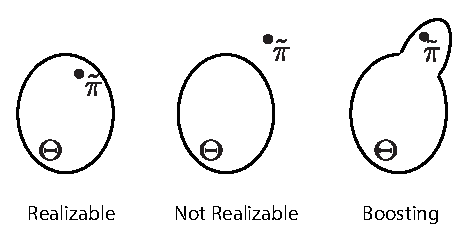
\includegraphics[width=0.5\textwidth]{f_figs/realizibility.eps}
\caption{
    \footnotesize
An illustration of the  of realizable. Denote a policy class $\Theta$ and a supervisor policy $\tilde{\pi}$, the supervisor's policy is realizable if it is contained in $\Theta$. We also illustrate Boosting, which can be thought of as adding to the function class to achieve realizability.}
\vspace*{-20pt}
\label{fig:teaserl}
\end{figure}


This insight and recent results in Machine Learning~\cite{krizhevsky2012imagenet} encourage us to reconsider these results. The underlying concern with the loss minimization approach was that the error would grow quadratically in time $O(T^2\epsilon)$. This is only problematic if $\epsilon$ is large, but suppose we could choose a richer class of controllers to very nearly match the supervisor’s policymaking $\epsilon$ very small. This is increasingly possible with Deep Neural Networks~\cite{anthony2009neural} that can in principle approximate any function given enough data and the ability to minimize training loss. Similarly, techniques like Boosting can incrementally enlarge the class of functions by training a sequence of sub-policies each focused on examples that caused the previous policy to fail and then uses a weighted combination of all trained policies~\cite{mason1999boosting}.

Using these rich function classes we are able to include the expected supervisor's policy in the robot's policy class. In this situation, which we refer to as realizable, the passive LfD approach can be guaranteed to achieve the supervisor's policy if enough data is collected. Thus, our contribution is to instead of considering the problem of distribution mismatch, we look at how at how function complexity affects the performance of DAgger and passive LfD. 


We  provide experiments in a gridworld domain demonstrating the effect of growing the robot's policy function class size and demonstrate that adaptivity may only be effective when the function class size is smaller than the supervisor's. We then illustrate a 2D point mass example, in which despite having the same function class as the supervisor adaptivity fails to converge to the supervisor's policy. Finally, we test both DAgger and passive Lfd in learning a policy for singulating objects from a pile on a Zymark Robot platform across 10 human subjects. We found the passive LfD is able to achieve a $21 \%$ increase in the probability of success with the same amount of data \mlnote{We will probably be able to increase that with boosting}


\section{Related Work}
Below we summarize related work in adaptive approaches in applications of Online LfD to robotics, sample complexity results and then work on reducing samples. \mlnote{Will update related work}


\noindent \textbf{Online LfD with an Expert Supervisor}
Online Learning from Demonstration in robotics has achieved numerous examples of completely model-free learning from high dimensional state representations, such as images. Successful robotic examples of Online Learning From Demonstration with an expert supervisor include applications to flying a quad-copter through a forest where the input is only image data taken from an on board sensor. 

Recently, Laskey et al. applied Online Learning from Demonstration to manipulation tasks such as surgical needle insertion \cite{laskeyshiv}, where a surgical robot correctly learns to insert a needle into tissue to prepare for suturing. Furthermore, Laskey et al. applied Online LfD to robotic de-cluttering, where a robot is given image data of a table with a variety of objects on it and must learn to push the obstacle objects aside to grasp a goal \cite{laskeyrobot}. 

Other succesful examples have been teaching a robotic wheel chair navigate to goal positions in the presence of obstacles and teaching a robot to follow verbal instructions to navigate across an office building \cite{kim2013maximum, duvallet2013imitation}. 

\noindent \textbf{Sample Complexity in Online LfD}
Sample complexity analysis in Online LfD is normally summarized as to results.  Ross et al. showed that a supervise learning approach (i.e. where no iterative online feedback is used) achieves an error rate that is quadratic in the time horizon, but is only an asymptotic bound \cite{ross2010efficient}. 

Ross et al. then models an iterative Online LfD algorithm known as DAgger as a Follow-The-Leader algorithms and gives regret bounds for strongly convex loss functions, however it also have linear dependence on $T$. We argue that both of these approaches can instead by thought of as traditional supervise learning, where the sample distribution is simply different than the distribution optimized over and model the problem as supervise learning with importance sampling weights. 

Finally of interest to us is the comparison to Reinforcement Learning methods. A common approach in RL for robotics is policy gradients, where a gradient is computed on the loss function based on sample estimates. Kakade et al. demonstrated that  a single gradient estimate can require on the order of cubic in the time horizon samples~\cite{kakade2003sample}. For perspective a robotic task has hundreds of time steps and can sometimes take minutes to sample a trajectory.

\noindent\textbf{Reducing Supervisor Burden in Online LfD} 
An interesting line of work in this field is applying active learning to the task of Online LfD, which has the promise to help reduce sample complexity. Active learning approaches to reducing supervisor burden only ask for supervision when the robot is uncertain about the
correct control to apply. Traditional active learning techniques like query-by-committee and uncertainty sampling have
been utilized for this purpose \cite{chernova2009interactive,judah2011active,grollman2007dogged}
Kim et al. demonstrated that due to the non-stationarity of the distribution of states encountered during
learning, the traditional active learning techniques may not be suitable.
Thus the use of novelty detection was proposed~\cite{kim2013maximum}. Laskey et al. introduced SHIV, using an active
learning approach tailored to high dimensional and non-stationarity state distributions and a modified version of the
One Class SVM classifier. This reduced the density estimation problem to a 
simpler regularized binary classification~\cite{laskeyshiv}. 


\section{Problem Statement}\label{sec:PS}
The goal of this work is to learn a policy that matches that of the supervisor's while asking the supervisor for as few examples as possible.

\noindent\textbf{Modeling Choices and Assumptions}  We model the system dynamics as Markovian, stochastic, and stationary. Stationary dynamics occur when, given a state and a control, the probability of the next state does not change over time. 

We model the initial state as sampled from a distribution over the state space.
We assume a known state space and set of controls. We also assume access to a robot or simulator, such that we  can sample from the state sequences induced by a sequence of controls.   Lastly, we assume access to a supervisor who can, given a state, provide a control signal label. We additionally assume the supervisor can be noisy and imperfect, noting that the robot cannot surpass the level of performance of the supervisor. 

\noindent\textbf{Policies and State Densities.}
Following conventions from control theory, we denote by $\mathcal{X}$ the set consisting of observable states for a robot task, consisting, for example, of 
high-dimensional vectors corresponding to images from a camera, or robot joint angles and object poses in the environment.
We furthermore consider a set $\mathcal{U}$ of allowable control inputs for the robot, which can be discrete or
continuous. We model dynamics as Markovian, such that the probability of state $\mathbf{x_{t+1}}\in
\mathcal{X}$ can be determined from the previous state $\mathbf{x}_t\in\mathcal{X}$ and control input $\mathbf{u}_t\in
\mathcal{U}$: 
$$p(\bx_{t+1}|\bu_{t},\bx_{t}, \ldots, \bu_{0}, \bx_{0})=p(\bx_{t+1}|\bu_{t}, \bx_t)$$
We assume a probability density over initial states $p(\bx_0)$.
%We denote the probability density over the initial state also by $p:\mathcal{X}\to \mathbb{R}$. 

A trajectory $\hat{\tau}$ is a finite series of $T+1$ pairs of states visited and corresponding
control inputs at these states, $\hat{\tau} = (\mathbf{x}_0,\mathbf{u}_0, ...., \mathbf{x}_T,\mathbf{u}_T)$, where $\bx_t\in \mathcal{X}$
and $\bu_t\in \mathcal{U}$ for $t\in \{0, \ldots, T\}$ and some $T\in \mathbb{N}$.  
For a given trajectory $\hat{\tau}$ as above, we denote by ${\tau}$ the corresponding trajectory in state space,
${\tau} = (\bx_0,....,\bx_T)$.


A policy is a function $\pi: \mathcal{X} \to \mathcal{U}$ from states to control inputs. 
We consider a space of policies $\pi_{\theta}:\mathcal{X}\to \mathcal{U}$ parameterized by some $\theta\in \Theta$. Any such policy $\pi_{\theta}$ in an environment with probabilistic initial state density and Markovian dynamics
induces a density on trajectories of length $T+1$: $$p(\tau | \theta)=
p(\bx_0)\prod_{i=0}^{T-1}p(\bx_{t+1}|\bu_t,\bx_t)p(\bu_t|\pi_{\theta}(\bx_t))$$


While we do not assume knowledge of the distributions corresponding to: $p(\bx_{t+1}|\bx_t,\bu_t)$, $p(\bx_0)$, $p(\bx_t|
\theta)$ or $p(\bx|\theta)$, we assume that we have a stochastic real robot or a simulator such that for any state
$\bx_t$ and control $\bu_t$, we can sample the $\bx_{t+1}$ from the density $p(\bx_{t+1}|\bu_t,\bx_t)$. 
Therefore, when 'rolling out' trajectories under a policy
$\pi_{\theta}$, we utilize the robot or a simulator to sample the resulting stochastic trajectories rather than
estimating $p(\bx|\theta)$ itself.


\noindent\textbf{Objective.} The objective of  policy learning is to find a policy that minimizes some known cost function $C(\hat{\tau}) = \sum^T_{t=1} c(\bx_t,\bu_t)$ of a trajectory $\hat{\tau}$. The cost $c:\mathcal{X}\times \mathcal{U}\to \mathbb{R}$ is typically user defined and task specific. 
For example, in the task of inserting a peg into a hole, a function on distance between the peg's current and desired final state is used \cite{levine2015end}.  

In our problem, we do not have access to the cost function itself. Instead, we only have access to 
a supervisor that can achieve a desired level of performance on the task. The supervisor provides the robot an initial set
an initial set of $N$ stochastic demonstration trajectories $\lbrace \tilde{\tau}^1,...,\tilde{\tau}^N \rbrace$. 
which are the result of the supervisor applying this policy. This induces a training data set $\mathcal{D}$ of all state-control input pairs from the demonstrated trajectories.

We are interesting in determining what parameter $\theta$ generates the sample demonstrations from the supervisors policy. The question can be framed as maximizing the conditional likelihood of the sample demonstrations conditioned on a given parameter $\theta$. 

$$\underset{\theta}{\mbox{max}} \prod^N_{n=1} p(\bx_0,n) \prod^T_{t=1} p(\bx_{t+1,n}|\bx_{t,n},\bu_{t,n})p(\bu_t|\bx_t,\theta)$$

In solving this optimization it is common to optimize the conditional log-likelihood, which maintains the same solution but breaks up the product terms into sums. 

\begin{equation}\label{eq:m_likeli_obj}
\underset{\theta}{\mbox{max}} \sum^N_{n=1}\sum^T_{t=1}\mbox{log }p(\bu_t|\bx_t,\theta)
\end{equation}


We note that the dynamics and initial state distributions are dropped in this objective because they are conditionally independent of $\theta$, once the controls are observed. 

 Traditionally  Eq. \ref{eq:main_obj}, has been known as the surrogate loss to denote a difference between the true cost function. We will refer the to function $l : \mathcal{U} \times \mathcal{U} \rightarrow \mathbb{R}$ as the surrogate loss through out this paper. The surrogate loss can either be an indicator function as in classification or a continuous measure as indicated above.  This rewrites the objective as follows: 

\begin{equation}\label{eq:main_obj}
\hat{\theta} = \underset{\theta}{\mbox{argmin}} \sum^N_{n=1}\sum^T_{t=1} l(\bu_{n,t}, \pi_{\theta} (\bx_{n,t})).
\end{equation}


Due to model mismatch (e.g. not being realizable), or a limited amount of data, solving Eq. \ref{eq:main_obj} may not lead to $\tilde{\pi}$.  Thus leading to a mismeasure in the distribution trained on and tested on.  Prior work ~\cite{ross2010reduction}  proposed an iterative method that solves this problem by aggregating data to converge to a distribution induced by the robot's policy. We review this approach in Sec. \ref{sec:DAgger}.
 
\section{Passive LfD}
While DAgger handles the problem of model mismatch via optimizing on the distribution induced by the robot, we will instead assume realizability is achievable and leverage supervise LfD.  

\subsection{Passive LfD}
In passive LfD, $N$ demonstrations are collected from the supervisor's distribution $p(\tau|\tilde{\pi})$ and the following objective is minimized: 

$$\underset{\theta}{\mbox{min}} \: \frac{1}{M} \sum^N_{i=1} \sum^T_{t=1} l(\pi_{\theta}(\bx_{t,i}), \pi_{\theta^*}(\bx_{t,i}))$$

This objective is known as empirical risk minimization. If the supervisor's policy is not realizable though than pure passive learning could suffer in performance from not being adaptive. Thus, leveraging a larger function class can be used to remedy this situation. 

Increasing the function class size of a robot's policy can be done in several ways 1) is to use a large function class representation such a deep neural networks, which have seen a re-emergence in recent years~\cite{levine2015end} 2) is to alrogithimically inflate the function class using an approach known as boosting.

Boosting operates by examining the error, or misclassifications, in the current training set at each iteration, $k$. Then weights the points higher that are misclassified using a specified function $f$ and learns a new $\pi_{\theta_k}$ parameter on this distribution.  Then the robot policy is updated as $\pi_{\sum \theta} = \sum^K_{k=1} w_k \pi_{\theta_k}$, where the policy is now an ensemble of weaker policy representations~\cite{mason1999boosting}.


Since we know that $\tilde{\pi} \in \Theta$ and that we can find the best fit for $\tilde{\pi}$ given the observed examples. Then the only reason that $\hat{\theta} \neq \tilde{\pi}$ is because not enough examples from the supervisor have been collected. 

Understanding how much data is needed to learn a function, is a well studied problem known as sample complexity analysis~\cite{anthony2009neural}. In this literature they use different metrics to describe the complexity of a function class and show rates on which a given function class would converge to the real solution. We refer the reader to \cite{vapnik2013nature}, for a review of such topics. 

We are interested in the total cost along a trajectory with respect to a policy, $\pi_{\theta}$, which is defined as $J(\theta) = \sum^T_{t=1} l(\pi_{\theta}(\bx_{t}),\pi_{\theta^*}(\bx_{t}))$.  If we assume the surrogate loss $l$ is convex with respect to $\theta$ and bounded between $[0,1]$, then if $\theta \in \Theta$. \\

\begin{theorem}\label{thm:sup}
For a policy, $\theta^n$ found via passive LfD, from $n$ trajectories collected from the supervisor the following is true with probability at least $1- 2\mbox{exp} (-m\delta^2/8)$

$$E_{p(\tau|\theta^*)} J(\theta^n)\leq T( 2R_{\Theta}(Tn) + \delta+ \frac{1}{\sqrt{Tn}})$$\\

\end{theorem}

In this result, $R_{\Theta}$ corresponds to the Rademacher complexity of the given function class $\Theta$. The Rademacher complexity is a measure of much a function can fit to random noise, more complex function classes can fit better and thus leading to slower rates of convergence. It is interesting to not that in this bound $T$ controls how much data is added to each iteration, thus a longer time step trajectory can lead to faster convergence depending on the function class. 

A main take away from from this theorem  is that at a non-asymptotic rate of demonstrations the surrogate loss will be zero on the distribution of the supervisor, thus corresponding to exact agreement between robot and supervisor. The exact rate itself will vary as a function of Rademacher Complexity of $\Theta$. 

The above theorem though only shows that the policy converges in the limit of infinite samples, however we are interested in bounding the performance of a policy trained on only $n$ demonstrations. 

 Define $\theta^n = \underset{\theta}{\mbox{argmin}} \sum^n_{i=1} J(\theta)$   $\:\:\tau \sim p(\tau|\theta^*)$, where $l(\pi_{\theta}(\bx),\pi_{\theta^*}(\bx)) = ||\pi_{\theta}(\bx_{i,t}) - \pi_{\theta^*}(\bx_{i,t})||_2$.We note that the controls can be bounded and normalized such that the $l \in [0,1]$.  We are interested in the situation where the supervisor and robot policy are stochastic with a Normal Distribution (i.e. $p(\bu|\pi_{\theta}(\bx)) = \mathcal{N}(\pi_\theta(\bx),\sigma I)$. The following statement can be said: \\

\begin{theorem}
Given a policy $\theta^n$, the following is true 
$$E_{p(\tau|\theta^n)} J(\theta^n) \leq \big(\sqrt{T\frac{1}{4\sigma}}+1\big)E_{p(\tau|\theta^*)} J(\theta^n)$$\\
\end{theorem}
\begin{proof}
For convenience we will write $E_{p(\tau|\theta)} = E_{\theta}$ and $l(\theta,\bx) = l(\theta)$. 

\begin{align}
&E_{\theta^n} J(\theta^n) - E_{\theta^*} J(\theta^n) \\
&= T(\frac{1}{T}E_{\theta^n} J(\theta^n) -\frac{1}{T}E_{\theta^*} J(\theta^n)\\
&\leq  T\mbox{sup}_{\theta} |\frac{1}{T}E_{\theta_n}J(\theta) - \frac{1}{T}E_{\theta^*} J(\theta)|\\
&\leq  T| | p(\tau|\theta^n) - p(\tau|\theta^*)||_{TV}\\
&\leq T\sqrt{\frac{1}{2} D_{KL}(p(\tau|\theta^*),p(\tau|\theta^n))}
\end{align}

Line 5 bounds the expected loss over $\theta^n$ by taking the worst case value. Line 6 leverages the fact that the worst case loss is bounded by $1$ and the definition of Total Variational distance. Line 7 uses Pinsker's inequality. 


\begin{align}
&= T\sqrt{\frac{1}{2} E_{p(\theta^*)} \mbox{log} \frac{p(\tau|\theta^*)}{p(\tau|\theta^n)}}\\
&= T\sqrt{\frac{1}{2} E_{p(\theta^*)} \sum^T_{t=1}\mbox{log} \frac{p(\bu_t|\bx_t,\theta^*)}{p(\bu_t|\bx_t,\theta^n)}}\\
&= T\sqrt{\frac{1}{4\sigma} E_{p(\theta^*)} \sum^T_{t=1} ||\bu_t- \pi_{\theta^*}(\bx_t)||_2^2 - ||\bu_t- \pi_{\theta^n}(\bx_t)||_2^2}\\
&\leq T\sqrt{\frac{1}{4\sigma} E_{p(\theta^*)} \sum^T_{t=1}  ||\pi_{\theta^*}(\bx_t) - \pi_{\theta^n}(\bx_t)||_2^2}
\end{align}

Line 12,13,14 come from the definition of KL divergence our Markov assumption and the fact that the policies are stochastic with a normal distribution, respectively. Line 15 leverages triangle inequality. 

\begin{align}
&= T\sqrt{\frac{1}{4\sigma} E_{p(\theta^*)} \sum^T_{t=1}  l(\pi_{\theta^n}(\bx_t),\pi_{\theta^*}(\bx_t))^2}\\
&= T\sqrt{T\frac{1}{4\sigma}E_{p(x|\theta^*)} \sum^T_{t=1}  l(\pi_{\theta^n}(\bx_t),\pi_{\theta^*}(\bx_t))^2}\\
&=\sqrt{T\frac{1}{4\sigma}}E_{p(\theta^*)} \sum^T_{t=1}  J(\theta^n)
\end{align}

Line 12 uses the definition of our surrogate loss, $l$. Line 13 applies the definition of the expected state distribution used in Ross et al. \cite{ross2010reduction}. Line 14 simplifies the expression and return to the surrogate loss over the distribution on trajectories. 

\end{proof}
 
 The above theorem suggest that passive LfD can in fact achieve a rate that is $T\sqrt{T}$ and not $T^2$ as suggested by Ross et al. \cite{ross2010reduction,ross2010efficient} when using the expected state distribution.  Theorem 4.1 and 4.2 can combined to show convergence of the robot's policy as a function of samples. 


\section{DAgger}\label{sec:DAgger}
Ideally the solution for Eq. \ref{eq:main_obj}, $\hat{\theta}$ would be a sample estimate of $\tilde{\pi}$. However if $\tilde{\pi} \nsubseteq \Theta$ or is not realizable, then one approach is to try and agree with supervisor on the distribution induced by the robot's policy $p(\tau|\hat{\theta})$ because those are the states the robot is most likely to visit. 

A challenge occurs though when trying to fit a function that agrees with the supervisor on the distribution of states induced by the policy. The problem stems from not knowing what the distribution will be after the policy is optimized. To tackle this problem an iterative algorithm was proposed that under certain conditions converges to optimizing on the distribution induced by the policy. 


 \subsection{Algorithm}
Instead of  minimizing the surrogate loss, in Eq. \ref{eq:main_obj},  DAgger attempts to find the distribution the final policy will end up on. In the not realizible situation, this can help reduce surrogate loss. 
DAgger~\cite{ross2010reduction} attempts this by iterating two steps: 1)
computing the policy parameter $\theta$ using the training data $\mathcal{D}$ thus far, and 2) by executing the policy
induced by the current $\theta$, and asking for labels for the encountered states. 
 
\subsubsection{Step 1}
The first step of any iteration $k$ is to compute a $\theta_k$ that minimizes surrogate loss on the current dataset $\mathcal{D}_k=\{(x_i,u_i)|i\in\{1,\ldots,M\}\}$ of demonstrated state-control pairs (initially just the set $\mathcal{D}$ of initial trajectory demonstrations):

 \vspace{-1ex}
\begin{align}\label{eq:super_objj}
\theta_{k} = \underset{\theta}{\argmin} \: \sum_{i=1}^{M} \sum_{t=1}^T  l(\pi_{\theta}(\bx_{i,t}),\bu_{i,t}).
\end{align}

This can be observed as minimizing the empirical risk on the aggregate dataset of all examples seen so far, note that equal weight is giving to each example regardless of high likely they under the current policy~\cite{scholkopf2002learning}. 
 

 \subsubsection{Step 2}
The second step at iteration $k$, DAgger rolls out the current policy, $\pi_{\theta_{k}}$, to sample states that are likely under $p(\tau|\theta_{k})$.  For every state visited, DAgger requests the supervisor to provide the appropriate control/label. Formally, for a given sampled trajectory  $\hat{\tau} = (\bx_0,\bu_0,...,\bx_T,\bu_T )$, the supervisor provides labels $\tilde{\bu}_t$, where $\tilde{\bu}_t \sim \tilde{\pi}(\bx_t) + \epsilon$, where $\epsilon$ is a  zero mean noise term, for $t\in \{0, \ldots, T\}$.
The states and labeled controls are then aggregated into the next data set of demonstrations $\mathcal{D}_{k+1}$:
$$D_{k+1}=\mathcal{D}_k \cup \{(\bx_t,\tilde{\bu_t})|t\in\{0,\ldots,T\}\} $$

Steps 1 and 2 are repeated for $K$ iterations or until the robot has achieved sufficient performance on the
task\footnote{In the original DAgger the policy rollout was stochastically mixed with the supervisor, thus with
    probability $\beta$ it would either take the supervisor's action or the robots. The use of this stochastically mix
    policy was for theoretical analysis and in practice, it was recommended to set $\beta = 0$ to avoid biasing the
sampling~\cite{NIPS2014_5421,ross2010reduction}}.

\subsection{Analysis of DAgger}
Ross et al. propose analyzing DAgger as an online optimization problem~\cite{ross2010reduction}.  In online optimization a learner plays a game where at each iteration, it chooses a policy and receives a loss from an adversary.  In the LfD setting, the learner is the robot's policy and the adversary would be the loss on the distribution of states induced by the policy $E_{p(\tau|\theta)} l(\pi_{\theta}(\bx),\tilde{\pi}(\bx))$~\cite{shalev2011online}.

DAgger in this context is known as a Follow the Leader (FTL) algorithm. In FTL, the best policy is chosen on all previous seen losses, or the aggregate dataset in the LfD context. Their analysis shows that under the condition when the surrogate loss, $l$, is strongly convex with respect to $\theta$, their policy has a regret that converges to the best the policy could have done on all previous seen losses $\underset{\theta}{\min} \sum_{k=1}^K p(\tau|\theta_k)$. 

A bound in regret though though does not imply the robot will be able to generalize to the unseen data nor match the supervisor. For example consider, where a robot is learning to search down a tree to maximize cumulative reward, as illustrated in Fig. \ref{fig:c_ex}. Here the robot's policy class is the finite set of only being able to choose left or right, $\Theta = \lbrace L,R \rbrace$.

\begin{figure}
\centering
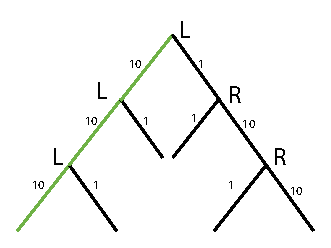
\includegraphics{f_figs/counter_exmp.eps}
\caption{
    \footnotesize
A binary decision tree, where a robot is being taught by a supervisor to descend down and achieve maximum cumulative reward, which is shown via the numbers on each branch. Each node has the action the supervisor would select, either left or right, $\lbrace L, R \rbrace$. The optimal policy, colored in green, is to select left, $L$, at each node.}
\vspace*{-20pt}
\label{fig:c_ex}
\end{figure}

The learning algorithm, which chooses how to update the policy is to choose the policy, which agrees with the supervisor's controls the most, or: 

$$\pi_{\theta} = \underset{\lbrace L,R \rbrace}{\mbox{argmin}} \sum^M_{m=0}\sum^T_{t=0} I(\pi_\theta(x_{m,t}),\tilde{\pi}(x_{m,t}))$$

If passive LfD is applied to this situation, the supervisor will always chose left, $L$, and the robot will select this action resulting in perfect imitation. However, if DAgger is used and the robots initial policy is to go right, $\pi_{\theta_0} = R$. Then the robot will repeatedly always choose right and never converge. 

Thus, convergence in regret is achievable because the best the robot could have done in hindsight would be to always choose $R$, but that does not result in a good policy. We note that if passive LfD was applied the robot would have chosen $L$ from the a single initial demonstration. 

 While this problem can be overcomed by increasing the robot policy's function class, a larger function class could result in more data needed to learn the policy\cite{kakade2009generalization}.
 
Another potential downside of DAgger is that when the supervisor's policy is in the robot's policy class over the entire workspace. DAgger could potentially converge at a slower rate because it is requesting labels in uninformative states, as we show in Sec. \ref{sec:gdw}. We note though that it is possible for DAgger to act as an active learning algorithm and query states near a policies decision boundary. This depends on the environment's dynamics and the robot's policy representation. 





\section{Experiments}

\begin{figure*}
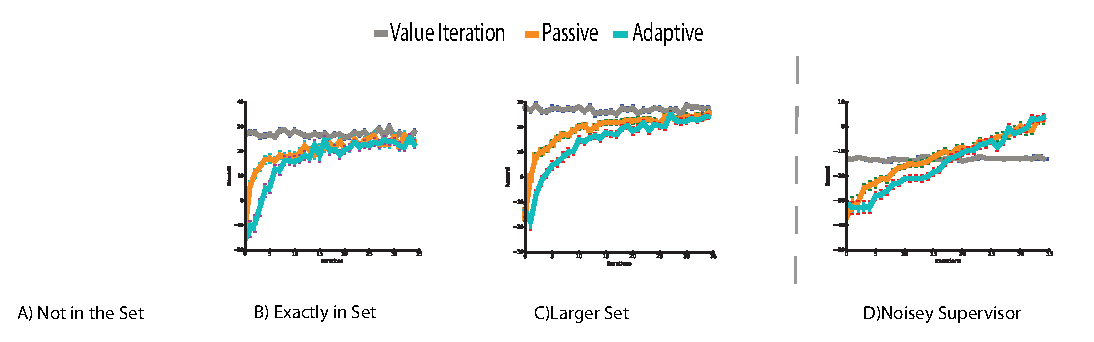
\includegraphics{f_figs/var_grid.eps}
\caption{
    \footnotesize
Shown above is the expected reward obtained for four different conditions in a 3D gridworld environment, where the robot is taught to avoid negative reward states and reach a goal state. Condition A examines when the robot's policy class is not able to learn the supervisors, which results in adaptivity leading to better performance. Condition B examines Boosting being used to incrementally increase the robot's policy class such that it contains the supervisor policy. Thus resulting in passive leading to faster convergence. Condition C examines a large robot policy class that is also able to represent the supervisor. This leads to similar performance as Condition B, but requires more data. Finally, Condition D examines when the supervisor has noise added to the controls labels, this leads to more data being needed to converge but the passive approach is still able to outperform adaptive.  }
\vspace*{-20pt}
\label{fig:var}
\end{figure*}

We provide experiments in a simulated GridWorld environment, which allows for us to vary noise in the dynamics and initial state distribution: $p(\bx_t|\bx_t,\bu_t)$ and $p(\bx_0)$, with a deterministic supervisor. Then we  train a Zymark robot to singulate objects from each other, which allows for us to look at high dimensional image environments and work with a human supervisor. 

\subsection{GridWorld}\label{sec:gdw}
In a simulated GridWorld, we have a point robot that is trying to reach a goal state, at which it receives $+10$ reward. The robot receives $-10$ reward if it touches a red state, as shown in Fig. \ref{fig:grid_world}. The robot has a state space of $(x,y)$ coordinates and a set of actions consisting of $\lbrace$LEFT,RIGHT,FORWARD,BACKWARD,UP,DOWN NONE$\rbrace$, where NONE indicates staying at the current stop. For the transition dynamics $p(\bx_{t+1}|\bx_{t},\bu_t)$, the robot goes to an adjacent state that does not correspond to the intended control with probability $0.2$. 

We use Value Iteration to compute an optimal supervisor for our grid world domain. The optimal policy must learn to be robust to the noise in the dynamics, reach the goal state and then stay there. The robot policy is represented as a decision tree with a maximum depth of $3$ and is trained using Sci-Kit Learn~\cite{scikit-learn}. We used a fix time horizon of $T=40$, which gives the robot enough time to get to the goal state. 


\noindent \textbf{Un-Realizable} In Fig. \ref{fig:var}, we show the case when the robot's policy class does not contain the supervisors, with a fixed decision tree of depth 3.  Similar to prior work passive LfD  with a fixed decision tree does worse than DAgger, which iteratively determines the distribution it policy induces and minimize the expected risk on it.

\noindent \textbf{Realizable} 
We then consider the situation where passive LfD and DAgger are able to to grow their function class via boosting, to place the supervisor's policy inside of it. To achieve this we applied AdaBoost to the decision trees from before and terminated the number of iterations once the training loss was zero. 

As shown in Fig. \ref{fig:var}, DAgger and passive LfD both converge to the supervisor, but more data is needed for DAgger. This suggests that adaptivity forces the robot to ask for uninformative demonstrations.  


\noindent \textbf{Over Realizable}
We next consider the situation where passive LfD and DAgger have a very large function class To achieve this we  set the robot;s policy, $\pi_{\theta}$ to the decision trees with a depth of $100$.

As shown in Fig. \ref{fig:var}, DAgger and passive LfD both converge to the supervisor, but in comparison to the Boosted decision trees more data is needed to converge to the supervisors. Thus, suggesting that using a larger than needed function class is prone to requiring more data. 

\noindent \textbf{Noisy Supervisor}
We finally observe the effects of noise on the supervisor. Here we consider the case where noise is applied to observe label, thus the robot recieve control labels that are $\bu = \pi_{\theta}(\bx) + \epsilon$, \mlnote{will fix that} where epsilon is an i.i.d distribution that selects a random control with probability $0.2$.

We use the large decision tree which is most susceptible to the noisy supervisor and observe the effects of passive LfD versus adaptive. As shown, both passive and adaptive are able to surpass the noisy supervisor's performance because they can average out the noise in the labels with enough data. Though it takes both substantially more data, passive LfD is able to achieve gains over adaptive. 




\subsection{Point Mass Control}
We next consider the example where the robot needs to learn to get to a location in a 2D continuous world domain. The robot is represented as a point mass dynamics and the supervisor is computed using the infinite time horizon LQG, which results in a linear policy. 

The domain, as shown in Fig. \ref{fig:p_mass}, consists of two areas A and B., which contain different dynamics and thus two different solutions to the LQG supervisor. In region B the controls are inverted between $x$ and $y$.  The goal state is located in area A. The robot's policy, $\pi_{\theta}$ is represented as a linear policy which is found via ridge regression. 

We run passive Lfd and DAgger in this setting and plot the performance in Fig. \ref{fig:p_mass}. As shown, passive LfD is able to converge to the true supervisor's policy however the adaptivitiy of DAgger forces it to enter the region B of the workspace and subsequently try to learn the two different supervisors. Thus, preventing it from converging. 

\begin{figure}
\centering
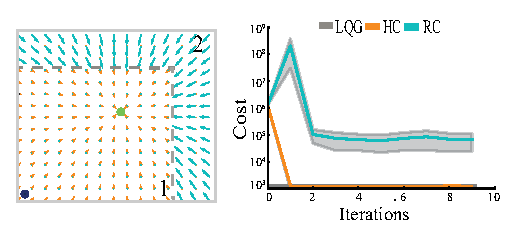
\includegraphics{f_figs/p_mass.eps}
\caption{
    \footnotesize
Left: A 2D workspace where a point mass robot is taught to go to the green circle starting from the blue circle. The world is divided into to two quadrants A and B, in B the controls are inverted in the dynamics thus resulting in $x=y$ and $y=x$. The supervisor is the infinite horizion LQG computed policy, which results in two different linear matrices in region A and B. Right: Illustrates how having a linear robot policy class can cause DAgger to fail  to converge due to it collecting data from region B.  }
\vspace*{-20pt}
\label{fig:p_mass}
\end{figure}

\subsection{Planar Singulation}
We lastly perform a human study on a real robot, where people teach the robot to perform singulation task, or seperate a object from a pile. The objects used to form clutter are red extruded polygons.  For singulation task, we consider objects made of Medium Density Fiberboard with an average 4" diameter and 3" in height. 

The robot has a 2 dimensional internal state of base rotation and arm extension. The state space of the environment, $\mathcal{X}$, is captured by  an overhead Logitech C270 camera, which is positioned to capture the workspace that contains all cluttered objects, the goal object and the robot arm. We use only the current image as state space, which captures positional information and a neural network architecture policy representation, the same as in~\cite{laskeyrobot}.

The robot is commanded via position 
control with a  PID controller. Similar to \cite{laskeyshiv}, the controls, $\mathcal{U}$, to the robot are bounded changes in the internal state, which allows for us to easily register control signals to the demonstrations provided by supervisors as opposed to torque control. The control signals for each degree of freedom are continuous values with the following ranges: base rotation, $[-15^\circ,15^\circ]$, arm extension $[-1,1]$. The units are degrees for base rotation and centimeters for arm extension. 

During training and testing the initial state distribution $p(\bx_0)$ consists of sampling the relative pose of 4 objects from a distribution around their position in the pile and the pose of the pile as a whole. The pose of the pile is sampled from a Gaussian with variance \mlnote{get numbers}. Then using a virtual overlay a human is asked to place objects in their correct pose. 

The robot can be trained in either 2 ways DAgger or passive learning. In passive learning, the subject is asked to provide 60 demonstrations to the robot using an Xbox Controller. In active learning the user is first asked to provide 20 demonstrations via the Xbox Controller and then provides retro-active feedback for $K=2$ iterations of 20 demonstrations each. 

10 human subjects were selected who had a background in robotics research, but not in LfD. They were given a short demonstration of the learned robot policy and then asked to practice providing feedback through DAgger for 5 demonstrations and passive for 5 demonstrations. We then have each subject provide the first 20 demonstrations via passive feedback and then using counter-balancing to select whether they will perform passive or DAgger for the next 40 demonstrations.  

In Fig. \ref{fig:izzy_rw} , we show the average performance of the policies trained with DAgger and passive LfD. Each policy is evaluated on a hold out set of 30 initial states sampled from the same distribution as training. As shown, the policies learned with DAgger exhibit statistically significant worse performance than those with passive LfD. Thus, sugggesting that DAgger could perform worse than passive Lfd on a task with actual human supervision. 

\begin{figure}
\centering
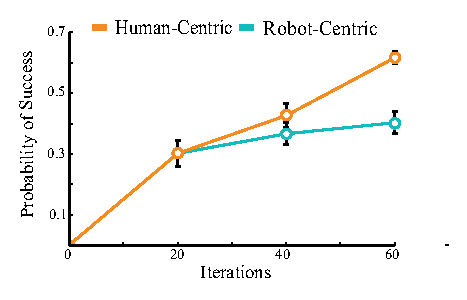
\includegraphics{f_figs/izzy_reward.eps}
\caption{
    \footnotesize
Shown is averaged success at the singulation task over the 10 human subjects. Each policy is evaulated 30 times on the a held out set of test configurations. The first 20 rollouts are from the supervisor rolling out there policy and the next 40 are collected via retro-active feedback for adaptive and tele-operated demonstrations for passive. Passive LfD shows a 20$\%$ improvement in success at the end. }
\vspace*{-20pt}
\label{fig:izzy_rw}
\end{figure}




  



\section{Conclusion}
\mlnote{This is specific to the theoretical analysis section}
In conclusion, we have shown that by knowing what distribution the robot is likely to encounter we can achieve more representative bounds on the performance of our policy. 

By achieving the familiar bound of Rademacher Complexity, we can now apply techniques such as Metric Entropy, Fat Shattering and VC Dimension to achieve sample complexity terms for both convex class and non-convex, which can be more enlightening than the previous FTL analysis. 

However, the bounds show a strong dependence on how large the importance sampling weights can become. This implies that if our policy starts to deviate from the training set during its empirical risk minimization. It is likely that the effective sample size could be quite low and thus require more samples. We present several ways to control for this factor and will begin experimentally seeing the effects.  

\bibliographystyle{IEEEtranS}
\bibliography{references}


\end{document}